\section{Definition of polygons}
\subsection{Defining the points of a square} \label{def_square}
We have seen the definitions of some triangles. Let us look at the definitions of some quadrilaterals and regular polygons.

\begin{NewMacroBox}{tkzDefSquare}{\parg{pt1,pt2}}%
The square is defined in the forward direction. From two points, two more points are obtained such that the four taken in order form a square. The square is defined in the forward direction. \\The results are in \tkzname{tkzFirstPointResult} and \tkzname{tkzSecondPointResult}.\\
We can rename them with \tkzcname{tkzGetPoints}.

\medskip
\begin{tabular}{lll}%
\toprule
Arguments             & example & explanation                         \\ 
\midrule
\TAline{\parg{pt1,pt2}}{\tkzcname{tkzDefSquare}\parg{A,B}}{The square is defined in the direct direction.}
\end{tabular}
\end{NewMacroBox}

\subsubsection{Using \tkzcname{tkzDefSquare} with two points}
Note the inversion of the first two points and the result.

\begin{tkzexample}[latex=4cm,small]
\begin{tikzpicture}[scale=.5]
  \tkzDefPoint(0,0){A} \tkzDefPoint(3,0){B}
  \tkzDefSquare(A,B)
  \tkzDrawPolygon[new](A,B,tkzFirstPointResult,%
               tkzSecondPointResult)
  \tkzDefSquare(B,A)
  \tkzDrawPolygon(B,A,tkzFirstPointResult,%
               tkzSecondPointResult) 
\end{tikzpicture} 
\end{tkzexample}

 We may only need one point to draw an isosceles right-angled triangle so we use \\ \tkzcname{tkzGetFirstPoint} or \tkzcname{tkzGetSecondPoint}.

\subsubsection{Use of \tkzcname{tkzDefSquare} to obtain an isosceles right-angled triangle}
\begin{tkzexample}[latex=7cm,small]
\begin{tikzpicture}[scale=1]
  \tkzDefPoint(0,0){A}
  \tkzDefPoint(3,0){B}
  \tkzDefSquare(A,B) \tkzGetFirstPoint{C}
  \tkzDrawSegment(A,B)
  \tkzDrawSegments[new](A,C B,C)
  \tkzMarkRightAngles(A,B,C)
  \tkzDrawPoints(A,B) \tkzDrawPoint[new](C)
  \tkzLabelPoints(A,B)
  \tkzLabelPoints[new,above](C)
\end{tikzpicture}
\end{tkzexample}

\subsubsection{Pythagorean Theorem and \tkzcname{tkzDefSquare} }
\begin{tkzexample}[latex=8cm,small]
\begin{tikzpicture}[scale=.5]
\tkzDefPoint(0,0){C}
\tkzDefPoint(4,0){A}
\tkzDefPoint(0,3){B} 
\tkzDefSquare(B,A)\tkzGetPoints{E}{F} 
\tkzDefSquare(A,C)\tkzGetPoints{G}{H} 
\tkzDefSquare(C,B)\tkzGetPoints{I}{J} 
\tkzDrawPolygon(A,B,C) 
\tkzDrawPolygon(A,C,G,H) 
\tkzDrawPolygon(C,B,I,J) 
\tkzDrawPolygon(B,A,E,F) 
\tkzLabelSegment(A,C){$a$} 
\tkzLabelSegment[right](C,B){$b$} 
\tkzLabelSegment[swap](A,B){$c$} 
\end{tikzpicture}
\end{tkzexample}

\subsection{Defining the points of a rectangle}
.

\begin{NewMacroBox}{tkzDefRectangle}{\parg{pt1,pt2}}%
The rectangle is defined in the forward direction. From two points, two more points are obtained such that the four taken in order form a rectangle. The two points passed in arguments are the ends of a diagonal of the rectangle. The sides are parallel to the axes.\\
 The results are in \tkzname{tkzFirstPointResult} and \tkzname{tkzSecondPointResult}.\\
We can rename them with \tkzcname{tkzGetPoints}.

\medskip
\begin{tabular}{lll}%
\toprule
Arguments             & example & explanation                         \\ 
\midrule
\TAline{\parg{pt1,pt2}}{\tkzcname{tkzDefRectangle}\parg{A,B}}{The rectangle is defined in the direct direction.}
\end{tabular}
\end{NewMacroBox}

\subsubsection{Example of a rectangle definition}
\begin{tkzexample}[latex=7 cm,small]
\begin{tikzpicture}
\tkzDefPoints{0/0/A,5/2/C}
\tkzDefRectangle(A,C) \tkzGetPoints{B}{D}
\tkzDrawPolygon[fill=teal!15](A,...,D)
\end{tikzpicture}
\end{tkzexample}

\subsection{Definition of parallelogram} 

Defining the points of a parallelogram. It is a matter of completing three points in order to obtain a parallelogram.
\begin{NewMacroBox}{tkzDefParallelogram}{\parg{pt1,pt2,pt3}}%
\begin{tabular}{lll}%
\toprule
arguments &  default & definition  \\ 
\midrule
\TAline{\parg{pt1,pt2,pt3}}{no default}{Three points are necessary}
\bottomrule
\end{tabular}
\end{NewMacroBox}

From three points, another point is obtained such that the four taken in order form a parallelogram. 
\\ The result is in \tkzname{tkzPointResult}. \\
We can rename it with the name \tkzcname{tkzGetPoint}...


\subsubsection{Example of a parallelogram definition}

\begin{tkzexample}[latex=7 cm,small]
\begin{tikzpicture}[scale=1]
 \tkzDefPoints{0/0/A,3/0/B,4/2/C} 
 \tkzDefParallelogram(A,B,C) 
 % or   \tkzDefPointWith[colinear= at C](B,A) 
 \tkzGetPoint{D}
 \tkzDrawPolygon(A,B,C,D)
 \tkzLabelPoints(A,B) 
 \tkzLabelPoints[above right](C,D)
 \tkzDrawPoints(A,...,D)
\end{tikzpicture}
\end{tkzexample}


\subsection{The golden rectangle} 
 \begin{NewMacroBox}{tkzDefGoldenRectangle}{\parg{point,point}}%
The macro determines a rectangle whose size ratio is the number $\Phi$.\\
 The created points are in \tkzname{tkzFirstPointResult} and \tkzname{tkzSecondPointResult}. \\
 They can be obtained with the macro \tkzcname{tkzGetPoints}. The following macro is used to draw the rectangle.

\begin{tabular}{lll}%
\toprule
arguments             & example & explanation                         \\
\midrule
\TAline{\parg{pt1,pt2}}{\parg{A,B}}{If C and D are created then $AB/BC=\Phi$.}
 \end{tabular}
 
 \tkzcname{tkzDefGoldenRectangle} or  \tkzcname{tkzDefGoldRectangle}
\end{NewMacroBox}


\subsubsection{Golden Rectangles}
\begin{tkzexample}[latex=6 cm,small]
\begin{tikzpicture}[scale=.6]
 \tkzDefPoint(0,0){A}      \tkzDefPoint(8,0){B}
 \tkzDefGoldRectangle(A,B) \tkzGetPoints{C}{D}
 \tkzDefGoldRectangle(B,C) \tkzGetPoints{E}{F}
 \tkzDefGoldRectangle(C,E) \tkzGetPoints{G}{H}
 \tkzDrawPolygon(A,B,C,D)
 \tkzDrawSegments(E,F G,H)
\end{tikzpicture}
\end{tkzexample}

\subsubsection{Construction of the golden rectangle }
Without the previous macro here is how to get the golden rectangle.

\begin{tkzexample}[latex=8cm,small]
\begin{tikzpicture}[scale=.5] 
\tkzDefPoint(0,0){A}
\tkzDefPoint(8,0){B} 
\tkzDefMidPoint(A,B)
\tkzGetPoint{I} 
\tkzDefSquare(A,B)\tkzGetPoints{C}{D} 
\tkzInterLC(A,B)(I,C)\tkzGetPoints{G}{E} 
\tkzDefPointWith[colinear= at C](E,B) 
 \tkzGetPoint{F}
\tkzDefPointBy[projection=onto D--C ](E) 
 \tkzGetPoint{H}
\tkzDrawArc[style=dashed](I,E)(D)
\tkzDrawPolygon(A,B,C,D) 
\tkzDrawPoints(C,D,E,F,H) 
\tkzLabelPoints(A,B,C,D,E,F,H)
\tkzLabelPoints[above](C,D,F,H)  
\tkzDrawSegments[style=dashed,color=gray]%
(E,F C,F B,E F,H H,C E,H) 
\end{tikzpicture}
\end{tkzexample}




\subsection{Regular polygon} 
 \begin{NewMacroBox}{tkzDefRegPolygon}{\oarg{local options}\parg{pt1,pt2}}%
From the number of sides, depending on the options, this macro determines a regular polygon according to its center or one side.

\begin{tabular}{lll}%
\toprule
arguments             & example & explanation                         \\
\midrule
\TAline{\parg{pt1,pt2}}{\parg{O,A}}{with option \code{center}, $O$ is the center of the polygon.}
\TAline{\parg{pt1,pt2}}{\parg{A,B}}{with option \code{side}, $[AB]$ is a side.}
 \end{tabular}

\medskip
\begin{tabular}{lll}%
\toprule
options             & default & example                         \\
\midrule
\TOline{name}{P}{The vertices are named $P1$,$P2$,\dots}
\TOline{sides}{5}{number of sides.}
\TOline{center}{center}{The first point is the center.}
\TOline{side}{center}{The two points are vertices.}
\TOline{Options TikZ}{...}{}
\end{tabular} 
\end{NewMacroBox}

\subsubsection{Option \tkzname{center}}
\begin{tkzexample}[latex=7cm, small]   
\begin{tikzpicture}
  \tkzDefPoints{0/0/P0,0/0/Q0,2/0/P1}
  \tkzDefMidPoint(P0,P1) \tkzGetPoint{Q1}
  \tkzDefRegPolygon[center,sides=7](P0,P1)
  \tkzDefMidPoint(P1,P2) \tkzGetPoint{Q1}
  \tkzDefRegPolygon[center,sides=7,name=Q](P0,Q1)
  \tkzFillPolygon[teal!20](Q0,Q1,P2,Q2)
  \tkzDrawPolygon(P1,P...,P7)
  \foreach \j in {1,...,7} {%
  \tkzDrawSegment[black](P0,Q\j)}
\end{tikzpicture}
\end{tkzexample}

\subsubsection{Option \tkzname{side}}
\begin{tkzexample}[latex=7cm, small]   
\begin{tikzpicture}[scale=1]
    \tkzDefPoints{-4/0/A, -1/0/B}
    \tkzDefRegPolygon[side,sides=5,name=P](A,B)
    \tkzDrawPolygon[thick](P1,P...,P5)
\end{tikzpicture}
\end{tkzexample}
\endinput